
\section{Gravity Models}
\label{sec:gravity}

\tikzstyle{decision} = [diamond, draw, 
    text width=4.5em, text badly centered, node distance=3cm, inner sep=0pt]
\tikzstyle{block} = [rectangle, draw, 
   text centered, rounded corners, minimum height=2em]
\tikzstyle{line} = [draw, -latex']
\tikzstyle{cloud} = [draw, ellipse, node distance=4cm,
    minimum height=2em]
\begin{center}
\begin{tikzpicture}[auto, scale=2]
   \node[cloud, align=center,text width=2cm] (1) at (0,0) {Zone 1 \par$P_1=100$, $A_1=200$};
   \node[cloud, align=center,text width=2cm] (2) at (4,2) {Zone 2 \par$P_2=200$, $A_2=50$};
   \node[cloud, align=center,text width=2cm] (3) at (3,-1){Zone 3\par$P_3=100$, $A_3=150$};
    
   \draw (1) to node {$t_{12}=5$} node [swap]{}(2)
             (2) to node {$t_{23}=3$} node [swap]{}(3)
             (1) to node {$t_{13}=4$} node [swap]{}(3);
\end{tikzpicture}
\end{center}
The figure above\footnote{This problem is adapted from ``Urban Transportation
Planning'' by Michael D. Meyer and Eric J. Miller.} presents a simple three zone
system, the link travel times for this system (for internal trips, $t_{ii}=2$
globally), and the zonal productions and attractions. Assume a gravity model of
the form
\begin{equation}
 T_{ij}=\dfrac{P_iA_j^*(t_{ij})^{-b}}{\sum_{j'}A^*_{j'}(t_{ij})^{-b}}
\end{equation}
where $A_j^*$ is a ``modified attraction term'' defined by the
algorithm shown in Figure \ref{alg:attractions}. This algorithm ensures that
the predicted trips to a given zone equal the true zonal attractions
$A_j$. 


\begin{figure}[h] 
\begin{centering}   
\begin{tikzpicture}[node distance = 2cm, auto, scale=0.45]
   % place nodes
  \node [cloud](k1) {$k=1$};
  \node [block, below of=k1](A){$(A_j^*)_k=A_j$};
  \node [block, below
  of=A](T){$(T_{ij})_k=\dfrac{P_i(A_j^*)_k(t_{ij})^{-b}}{\sum_{j}(A^*_{j})_k(t_{ij'})^{-b}}$};
  \node [block, below
  of=T](A1){$(A_j^*)_{k+1}=(A_j^*)_k\dfrac{A_j}{\sum_i(T_{ij})}$};
  \node [block, below
  of=A1](choice){$|\sum_i\sum_j(T_{ij,k} - T_{ij,k-1})|\overset{?}{\le}\varepsilon$};
  \node [cloud, left of=A1](k+){$k=k+1$};
  \node [decision, below of=choice](done){Done};
  % Draw edges
  \path[line](k1)--(A);
  \path[line](A)--(T);
  \path[line](T)--(A1);
  \path[line](A1)--(choice);
  \path[line, dashed](choice)-| node [near start]{no}(k+);
  \path[line, dashed](k+)|-(T);
  \path[line](choice)-- node[near start]{yes}(done);
\end{tikzpicture}
\caption{Algorithm to match $A^*$ and $A$}
\label{alg:attractions}
\end{centering}
\end{figure}

Use Matlab or a similar programming software to write a program that computes
the O-D flows for this system using the algorithm (with $\varepsilon=1$). Find
the value of $b$ (to a single decimal place) which provides the ``best fit''
with the observed O-D matrix in Table \ref{tab:ODmatrix}. In your memo reporting
the results of this analysis, discuss how you determined which $b$ value gave
the ``best fit.''

\begin{table}[h!]
  \caption{Observed Origin-Destination flows for Problem \ref{sec:gravity}.}
	\label{tab:ODmatrix}
\begin{center}
\begin{tabular}{l c c c}
\hline
$i$ & 1 & 2 & 3\\
\hline
1 & 80 & 5 & 15\\
2 & 80 & 40 & 80\\
3 & 40 & 5 & 55\\
\hline
\end{tabular}
\end{center}
\end{table}

\subsection{Network Improvements}
The region represented in Problem 6.1 has begun improvements to the link between
zones 1 and 2 that will reduce the travel time from 5 to 3. Using your program
and the value of $b$ estimated above, determine the effect of this improvement
on the predicted trip distribution matrix.

\clearpage
\section{Lab}
The distribution models in the Wasatch Front model are not really good to 
experiment with, because the really interesting steps are done with a 
destination choice model, something we have not really covered in detail. So
instead of fiddling with the gravity model, we will use this week to show
you how to get more interesting data from Cube.

\subsection{Viper Files}
Cube makes it possible to visually inspect the attributes of a highway
network, by adjusting the color and thickness of lines based on rules you give
it. These rules can be saved as a ``viper'' file, with a \verb1.vpr1
extension. When you open a highway network in Cube, the software will try to
match a viper file from the current directory. So if you open \verb1foo.net1
Cube will try to find \verb1foo.vpr1 in that directory. If it can't find it,
it will try and find \verb1default.vpr1. If that fails, it will just do a
default color scheme, with blue links and grey TAZ connectors.\footnote{Note
that the Cube default is not necessarily the same as what you have in a default
viper file.}

From the Cube open file dialog, you can open either a highway network or a
viper file. If you open the viper file first, you can then view any highway
network using the layer manager. So you can develop a viper file with very
complex specifications and then use it for all of the model runs in a project.

To set the viper specifications, open a highway network file. Any network will
do, although you will typically use either the input highway network or a
loaded network post-assignment. If you have no other \verb1.vpr1 files in your
directory, you will get the Cube default, as shown in Figure
\ref{fig:defaultvpr}.

\begin{figure}[t]
\centering
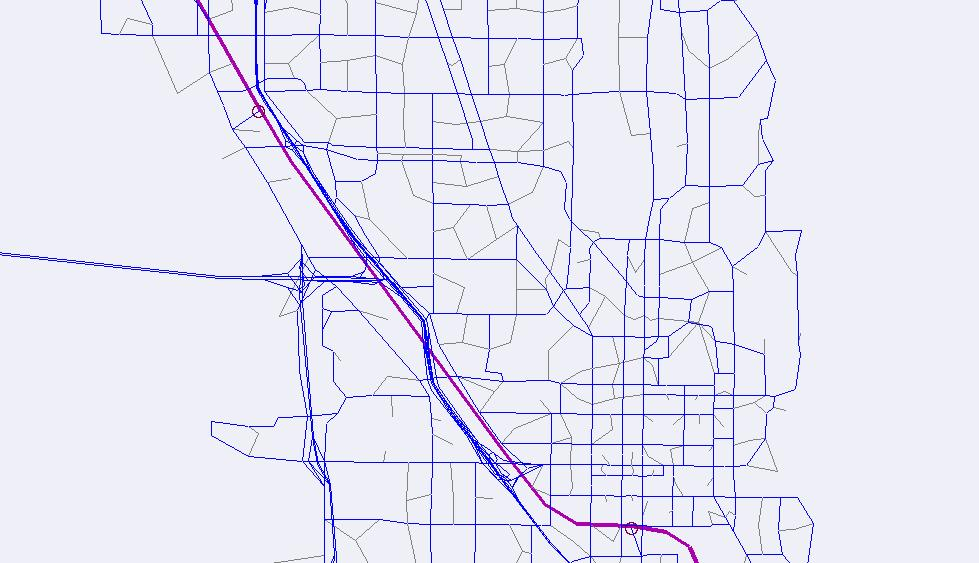
\includegraphics[width=\linewidth]{defaultvpr.JPG}
	\caption{Provo viewed with no viper specifications.}
	\label{fig:defaultvpr}
\end{figure}

The ``Home'' tab on the Cube menu bar contains several commands for displaying
the highway network and editing viper files. If you click on the linetypes and
colors on the ``Post Link'' box, you will get a dialog like the one shown in
Figure \ref{fig:linetypes}. You can change these definitions and save them as
group types. Clicking on the ``Color'' drop down tab in the same box will
allow you to quickly switch between color definitions. So you could have a
color definition for 2010 and 2030 functional types, or AM and PM volumes.
Similar tools are available for displaying node attributes. An example is
shown in Figure \ref{fig:2030vpr}.

\begin{figure}[t]
\centering
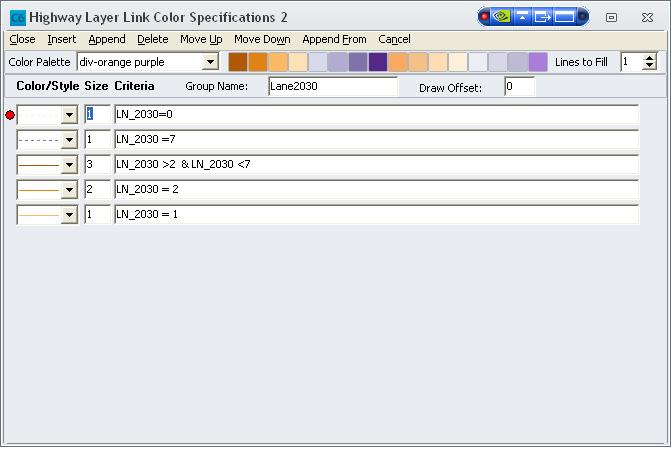
\includegraphics[width=\textwidth]{linetypes.JPG}
	\caption{The link specifications dialog box.}
	\label{fig:linetypes}
\end{figure}

\begin{figure}[t]
\centering
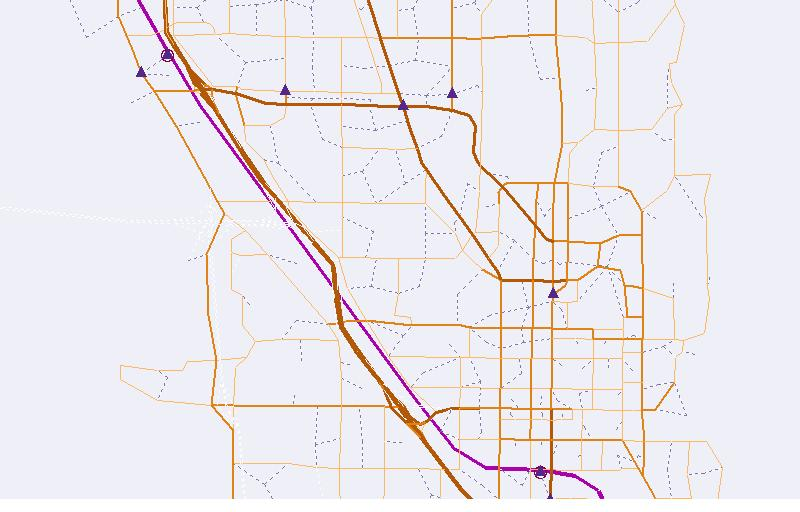
\includegraphics[width=\textwidth]{2030.JPG}
	\caption{Provo viewed with definitions showing 2030 lanes and park and ride
			lots.}
	\label{fig:2030vpr}
\end{figure}

The Wasatch Front travel demand model has a number of out-of-the box viper
files; unfortunately many of them have not been updated from model version 6,
and so require fields that are no longer in the model. You can save the viper
definitions you create by selecting
\verb1File -> Save As -> Project As1. 


\subsection{Desire Lines}
Many of the most important output files from the travel demand model are trip
matrices, showing where people travel to and from. Unfortunately, these are
extremely large files that are almost impossible for a human to read. So Cube
has tools to display these matrices on top of a highway network.

To do this, follow the steps outlined below.
\begin{enumerate}
\item{Open a trip distribution matrix. Perhaps the most comprehensive is the
\verb9AllTripsX100_pkok.mtx9 file which has all trip types
broken out by mode.}
\item{From your highway network click on ``Link to Matrix...'' on the
``Analysis'' tab. You will see a list of all your open matrix files. Select
the matrix you wish to analyze, click ``Add,'' and notice that your matrix has
been labeled ``M1=...'' Exit the dialog.}
\item{The ``Desire Lines ...'' command on the ``Analysis'' tab has now been
activated. Click this button to bring up the desire lines toolbar.}
\item{In the ``Matrix Table(s)'' field, enter \verb#M1.Tn# where \verb1n1 is
the number of the table you want to visualize. If we wanted to see all auto
trips on the \verb$AllTripsX100_pkok.mtx$ matrix, for instance, we would use
\verb#M1.T4#.}
\item{Set the scale to some number that makes sense. Cube will create a line
from $i$ to $j$ of one pixel width for each ``scale.'' That is, if we set the
scale at 5, then every 5 trips from $i$ to $j$ will add another pixel width.
This number will usually require some adjustment. Remember that in the
\verb$AllTripsX100$ matrix, a scale of 100 means one trip.}
\item{Set the ``Org Exp'' and ``Dest Exp'' zones to some value representing
the type of map you want. I typically look at one destination zone and all
origin zones in some geography.}
\item{Push ``Display.''}
\end{enumerate}
Figure \ref{fig:desires} shows desire lines for all auto trips to Brigham 
Young University with a scale of 30. Viewing transit trips is simply an issue
of changing the table definition.

\begin{figure}[t]
\centering
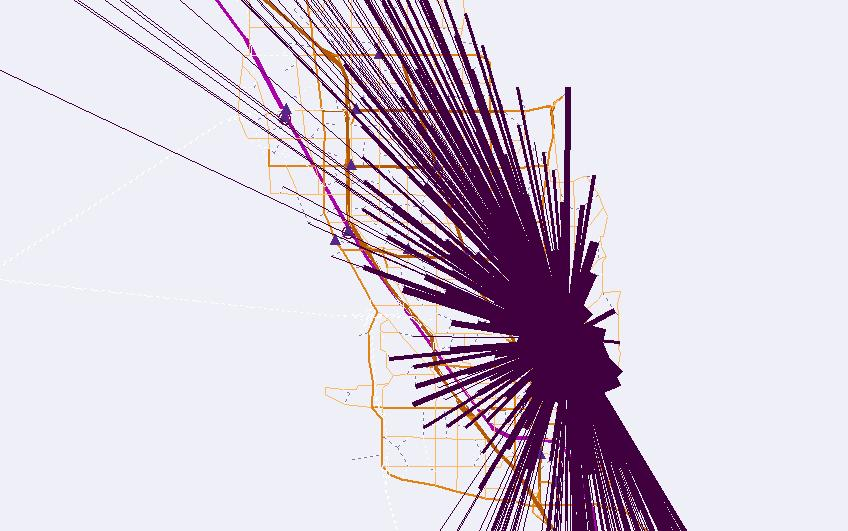
\includegraphics[width=\textwidth]{desirelines.JPG}
	\caption{Desire lines for automobile trips to Brigham Young University}
	\label{fig:desires}
\end{figure}

\subsection{GIS Integration}  
Cube is very much integrated with ArcGIS\footnote{In fact, you cannot buy Cube
without also buying a license for ArcGIS, a fact that keeps Cube
Windows-exclusive for now.}, and it is possible to use ArcGIS's capabilities to
produce truly beautiful data visualizations.

Cube has capabilities to create, edit, and view shapefiles within Cube itself,
but I usually find it less frustrating to just use ArcGIS some other GIS
engine.\footnote{I'm a big proponent of open source software, and Mac OS, so I
use QGIS.} At any rate, you will need to create a {\em personal geodatabase} to
store the geospatial information related to your projects. This is just a
repository to conveniently store binary or ASCII files (like the \verb1.NET1 and
\verb1.lin1) files in a way that can be projected in GIS software. To do this,
follow the steps below:
\begin{enumerate}
\item{Open the Data Manager in Cube by clicking on the cylinder-shaped button at
the top of the menu bar.}
\item{Right-click in the Data Manager window, and select "New Geodatabase"}
\item{Select where you would like the file stores, and how you want it named.
You may want a geodatabase for each project, or for each scenario, depending on
how much you are going to use it. Do not use spaces in the name.}
\item{The Create Data dialog will come up instantly. Set the spatial reference
to projected coordinate system 1983 NAD UTM Zone 12N.}
\item{You can add network and line files to this geodatabase using the
Import/Export Data dialog. These networks can now be projected in GIS software,
and you can add other non-Cube shapefiles to your maps.}
\end{enumerate}

When you have transit line files mapped in ArcGIS, you can join information on
the route ridership using the output dbf files in the mode choice directory,
though some data manipulation may be needed.

It is possible to add desire line information to a geodatabase map, but that is something I
will have to update later.

\subsection{Homework}
\paragraph{1. Viper File} Create a viper file that shows peak period
volume/capacity levels of service as colors.  Use the level of service
definitions given in Table \ref{tab:LOS}. In your memo, include a screenshot of
your Base 2009 scenario (zoomed in on some interesting geography) with your
definitions. Attach your \verb1los.vpr1 file to the assignment in T-square.

\paragraph{2. Desire Lines} Build desire line maps (screenshots are fine)
showing non-motorized trips to the University of Utah and Brigham Young
University. Build two more maps showing walk-access transit trips to both
schools. Comment on the distribution of trips to the two schools.


\paragraph{3. Data Visualization} Create a personal geodatabase in your
directory. Add the highway network and the 2030 rail files.  Create a map using
GIS software that shows the investment per rider on each segment of the rail
network in the 2030 base scenario (use an estimated \$7 per revenue mile).
Comment on what you see.

\begin{table}[ht]
	\caption{Level-of-Service Definitions}
	\label{tab:LOS}
\begin{center}
\begin{tabular}{l c c}
LOS & V/C & Color \\
\hline
A	& $\leq$ 0.34			& Blue \\
B	& 0.35 - 0.54 & Light Blue\\
C	& 0.55 - 0.77 & Green\\
D	&	0.78 - 0.93 & Yellow\\
E	& 0.94 - 0.99 & Orange\\
F	& $\geq$ 1.00   & Red\\
\hline
\end{tabular}
\end{center}
\end{table}
